Run-to-Completion and Pipeline are two models of execution for packet processing and forwarding at User Plane Function.
Comparison of these models in the different use cases/scenarios is one of the major objectives of our work. This chapter will explain these models of execution.

\section{Run-to-Completion (RTC) \label{secRTC} }
 \begin{figure}[htbp]
    \centering
    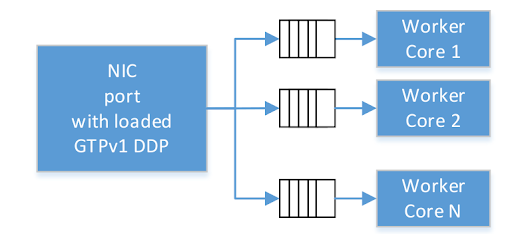
\includegraphics[width=0.7\textwidth, keepaspectratio]{./fig/ModelsofExecution/RTC.png}
    \caption{Run-to-Completion}
    \label{figRTC}
    \end{figure}
Keeping processors independent with minimal or no communication between them is the key idea of this model. Each
 processor should be able to completely recieve, process and forward/transmit the packet if required. Redirection of packets on different core requires receive side scaling (RSS) discussed in chapter \ref{chapterRSS}. Packets of a session are redirected to the same core as RSS value for packets of the same session is same.
\section{Pipeline \label{secPipeline}}
\begin{figure}[htbp]
    \centering
    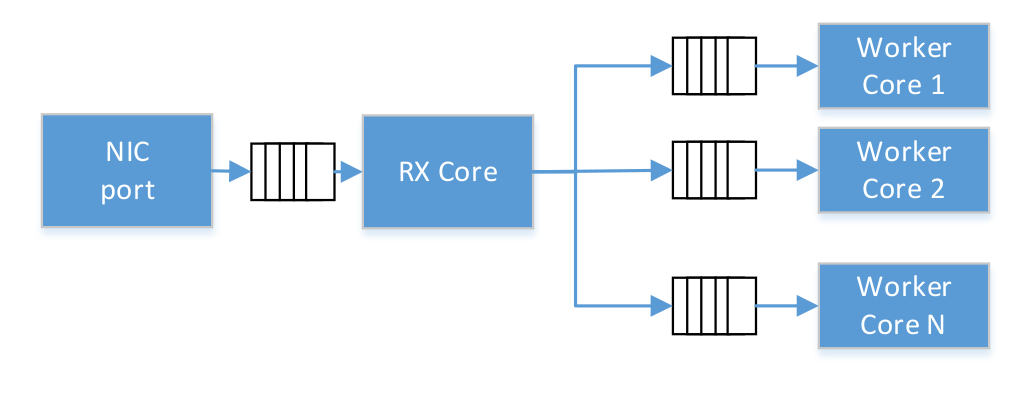
\includegraphics[width=0.7\textwidth, keepaspectratio]{./fig/ModelsofExecution/Pipeline.png}
    \caption{Pipeline}
    \label{figPipeline}
\end{figure}
 Hardware based redirection is either not possible or not used in this model. Complete packet processing including redirection occurs in software. Packets are redirected to a master core which processes the outer headers to redirect packet on one of the worker cores. Generally packets of a session are redirected to the same core to maintain better spatial and temporal locality. However packets may be redistributed if a particular core gets overloaded.
It requires inter-core communication. This communication happens through a software ring/circular queue for each worker core. The master core keeps incoming packets on the corresponding software ring of the worker core. The processed packets are then received by master core (through another ring) to transmit them over the wire.
The pipeline model can also redistribute load by shifting load from high load core to least loaded loead.
Our pipeline implementation handles this by mapping UEs from heavy loaded core to lightly loaded core. The UEs are remapped as long as there is no uniform distribution of load among different cores.
\section{Comparison \label{RTCpipelineComparison}}

The RTC has some significant advantages over the pipeline model.
\begin{itemize}
    \item \textbf{Better Throughput} The per core processing capability is expected to be higher in RTC model. This is due to no inter core communication and
 hardware support for hash computation. The computation in the hardware is generally faster than in software. This also keeps
  CPUs meant for hash computation free for other tasks. 
  \item \textbf{Lower Latency}The end to end latency in pipeline also takes a hit due to intercore
   communication between master and worker core.
\item \textbf{Easy to implement and understand} The RTC implementation's source code is easy to understand as it is same on all the cores. Pipeline has different logic and complex interaction between master and worker cores.
\end{itemize}
 
However, pipeline is better suited to change operational behavior dynamically. This hypothesis is tested for two use cases.
\begin{itemize}
    \item \textbf{Dynamic Scaling} The key idea here is to start user plane function with minimum number of cores and vary
     the number of cores according to the current traffic load. This helps in better energy efficiency as the cores may
      remain idle when there is less traffic. It  is easy to reconfigure the number of cores in pipeline than RTC. RTC
       requires stopping of ports before reconfiguring them as the number of RSS queues needs to be updated in hardware. A large number of packets are dropped during this reconfiguration. Pipeline requires the launch of cores in software which is relatively light weight.
    \item \textbf{Redistribution of traffic}  Once flows are mapped to cores by hash output in RTC, it is not possible to redirect them to another core. This may be required when the load is
     highly skewed towards some cores and the rest of the cores are idle. In such cases, a large number of packets are
      dropped by heavily loaded core in RTC model. 
    Pipeline can effectively handle such scenarios by redirecting certain flows from heavily loaded cores to less loaded cores. This reduces the number of packets dropped and better core utilisation. 
\end{itemize}

Experiments (discussed in chapter \ref{chapterExperimentsandResults}) were performed to test and evaluate these claims in 5G use case context. 
